
Question 2.3:\\	
\textsl{Select the features with the top 100 corresponding coefficient values (since this is a multi-class model, you can rank the coefficients using the maximum absolute value over classes, or the sum of absolute values). Take the evaluation training data in p2\_evaluation and use a subset of the genes consisting of the features you selected. Train a logistic regression classifier on this training data, and evaluate its performance on the evaluation test data. Report your score. (Don't forget to take the log transform $log_2(X+1)$ before training an testing.)}\\
\textsl{Compare the obtained score with two baselines: random features (take a random selection of 100 genes), and high-variance features (take the 100 genes with highest variance). Finally, compare the variances of the features you selected with the highest variance features by plotting a histogram of the variances of features selected by both methods.}\\

Answer:\\
We draw the 100 most important features (highest sum of absolute values within each feature) from the problem above. These features are used to choose the features from the new dataset. The score on the test data set is 0.153\footnote{The function parameters for \texttt{sklearn.linear\_model.LogisticRegression} were set in the same manner as in question 2.2.}.\\

By randomly choosing 100 features a score of 0.303 was achieved.\\

By choosing the 100 features of highest variance we can achieve a score of 0.924.\\

The first test score is very low due to a different setup of this problem compared with the problem above. One model has 3 clusters, whereas the new dataset has 36 different clusters. This has a great impact on the calculated labels and leads to the lowest score in this problem.\\

Choosing 100 features randomly leads to a higher score. But the highest score was achieved by choosing 100 features of highest variance. This makes sense, because the logic is comparable to the dimensionality reduction with PCA. Here we favor high PC's which represent high variances as well. The histograms show how far the variances of the second and the third approach are apart (see figure \ref{fig:historams_variance}). Thus the labels can be calculated more reliable in the case of higher variances.\\

\begin{figure}[h]
	\centering
	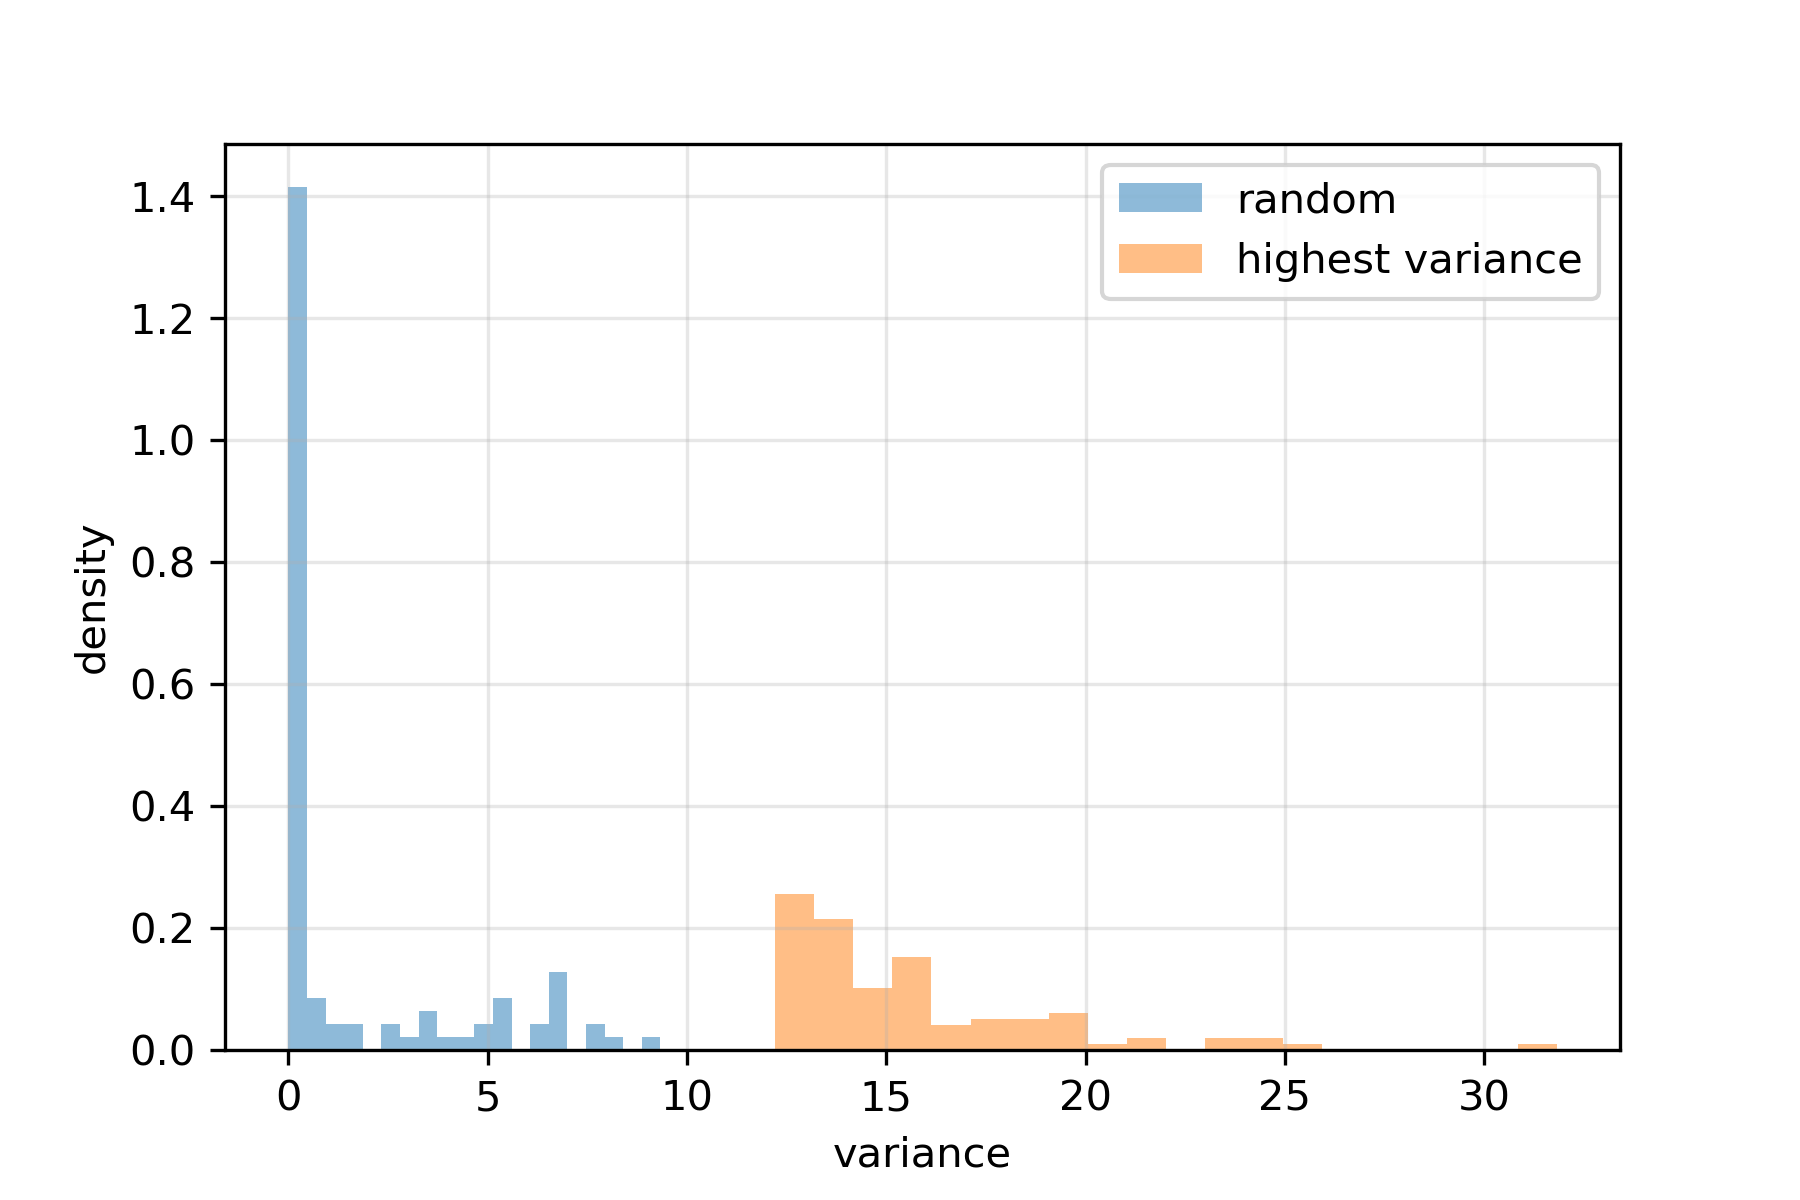
\includegraphics[width=0.7\linewidth]{problem_02/historams_variance}
	\caption{Histograms of 100 differently chosen features (integral sums to 1)}
	\label{fig:historams_variance}
\end{figure}